\section{Topología de la red MPLS}

La figura ~\ref{CON1} presenta la topología de la 
red MPLS utilizada en el proyecto. 
En esta topología, se puede observar la interconexión 
entre los routers y la Raspberry Pi, que actúa como 
un nodo de monitoreo para capturar y analizar el 
tráfico de la red mediante SNMP y Netdata.

\begin{figure}[H]
    \centering
    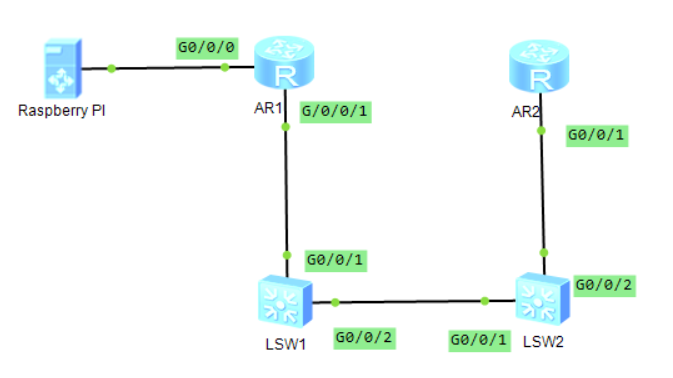
\includegraphics[scale= 0.9]{Pictures/RED.png}
    \caption{Topologia de la red MPLS}
    \label{CON1}

\end{figure}

Para que el servidor de monitoreo, en este caso la Raspberry Pi, pueda capturar y analizar el tráfico de la red, es necesario que pueda tener comunicación con todos los dispositivos de la red, para esto se configuró rutas estáicas en la Raspberry Pi, de tal manera que pueda alcanzar a todos los dispositivos de la red MPLS. Para eso, se modificó el archivo: sudo nano /etc/netplan/50-cloud-init.yaml 

Contenido del archivo:

\begin{lstlisting}[style=terminal]
network:
  version: 2
  ethernets:
    eth0:
      dhcp4: false
      dhcp6: false
      addresses:
        - 192.168.10.1/24
      routes:
        - to: 1.1.1.1/32
          via: 192.168.10.2
        - to: 2.2.2.2/32
          via: 192.168.10.2
        - to: 3.3.3.3/32
          via: 192.168.10.2
        - to: 4.4.4.4/32
          via: 192.168.10.2
\end{lstlisting}

Luego, se confirma la configuración de la red con el comando: 
\begin{lstlisting}[style=terminal]
sudo netplan try
\end{lstlisting}

La Raspberry Pi, probará la configuración de red y si todo está correcto, se aplicará la configuración de manera permanente, al presionar Enter. En caso de que la configuración no sea correcta, se revertirá a la configuración anterior.

Ahora, se debe de configurar netdata, para esto, se modifica el archivo respectivo de netdata, com se realizó en el caítulo 2.

\begin{lstlisting}[style=terminal]
jobs:
  - name: ar651_a
    hostname: 1.1.1.1
    update_every: 10
    timeout: 5
    options:
      options:
        version: 3
        max_repetitions: 5
        max_request_size: 1
        timeout: 10
        retries: 2
    user:
      name: netdata-user
      level: authPriv
      auth_proto: sha256
      auth_key: "NetAuth2026"
      priv_proto: aes
      priv_key: "NetPriv2026"

  - name: s6730h_c
    hostname: 2.2.2.2
    update_every: 10
    timeout: 5
    options:
      options:
        version: 3
        max_repetitions: 5
        max_request_size: 1
        timeout: 10
        retries: 2
    user:
      name: netdata-user
      level: authPriv
      auth_proto: sha256
      auth_key: "NetAuth2026"
      priv_proto: aes
      priv_key: "NetPriv2026"

  - name: s6730h_d
    hostname: 3.3.3.3
    update_every: 10
    timeout: 5
    options:
      options:
        version: 3
        max_repetitions: 5
        max_request_size: 1
        timeout: 10
        retries: 2
    user:
      name: netdata-user
      level: authPriv
      auth_proto: sha256
      auth_key: "NetAuth2026"
      priv_proto: aes
      priv_key: "NetPriv2026"

  - name: ar651_b
    hostname: 4.4.4.4
    update_every: 10
    timeout: 5
    options:
      options:
        version: 3
        max_repetitions: 5
        max_request_size: 1
        timeout: 10
        retries: 2
    user:
      name: netdata-user
      level: authPriv
      auth_proto: sha256
      auth_key: "NetAuth2026"
      priv_proto: aes
      priv_key: "NetPriv2026"
\end{lstlisting}

La implementación utiliza dos routers Huawei AR651 como dispositivos de
borde y dos switches Huawei S6730H como dispositivos de tránsito. La
configuración se divide en cuatro etapas: configuración del protocolo OSPF,
creación de un LSP estático, implementación de LDP y modificación del modo
de anuncio de etiquetas.

Antes de ejecutar los comandos se debe comprobar el nombre real de las
interfaces:

\begin{lstlisting}[style=terminal]
<HUAWEI> display interface brief
\end{lstlisting}

Los puertos Ethernet de los switches S6730H deben funcionar como interfaces
de capa 3. Para ello se utiliza el comando \texttt{undo portswitch}. Si el
comando no está disponible o la interfaz ya trabaja en capa 3, se puede
omitir.

\subsection{Configuración base y OSPF}

\subsubsection{Configuración de AR651-A}

\begin{lstlisting}[style=terminal]
<HUAWEI> system-view
[HUAWEI] sysname AR651-A

[AR651-A] interface GigabitEthernet0/0/1
[AR651-A-GigabitEthernet0/0/1] ip address 10.0.12.1 255.255.255.252
[AR651-A-GigabitEthernet0/0/1] undo shutdown
[AR651-A-GigabitEthernet0/0/1] quit

[AR651-A] interface LoopBack0
[AR651-A-LoopBack0] ip address 1.1.1.1 255.255.255.255
[AR651-A-LoopBack0] quit

[AR651-A] ospf 1
[AR651-A-ospf-1] area 0.0.0.0
[AR651-A-ospf-1-area-0.0.0.0] network 1.1.1.1 0.0.0.0
[AR651-A-ospf-1-area-0.0.0.0] network 10.0.12.0 0.0.0.3
[AR651-A-ospf-1-area-0.0.0.0] network 192.168.10.0 0.0.0.255
[AR651-A-ospf-1-area-0.0.0.0] quit
[AR651-A-ospf-1] quit
[AR651-A] return
\end{lstlisting}
Como se puede observar, se anuncia la red 192.168.10.0, la cual corresponde a la red de monitoreo donde se encuentra la Raspberry Pi, para que pueda tener comunicación con todos los dispositivos de la red MPLS.

\subsubsection{Configuración de S6730H-C}

\begin{lstlisting}[style=terminal]
<HUAWEI> system-view
[HUAWEI] sysname S6730H-C

[S6730H-C] interface GigabitEthernet0/0/1
[S6730H-C-GigabitEthernet0/0/1] undo portswitch
[S6730H-C-GigabitEthernet0/0/1] ip address 10.0.12.2 255.255.255.252
[S6730H-C-GigabitEthernet0/0/1] undo shutdown
[S6730H-C-GigabitEthernet0/0/1] quit

[S6730H-C] interface GigabitEthernet0/0/2
[S6730H-C-GigabitEthernet0/0/2] undo portswitch
[S6730H-C-GigabitEthernet0/0/2] ip address 10.0.23.1 255.255.255.252
[S6730H-C-GigabitEthernet0/0/2] undo shutdown
[S6730H-C-GigabitEthernet0/0/2] quit

[S6730H-C] interface LoopBack0
[S6730H-C-LoopBack0] ip address 2.2.2.2 255.255.255.255
[S6730H-C-LoopBack0] quit

[S6730H-C] ospf 1
[S6730H-C-ospf-1] area 0.0.0.0
[S6730H-C-ospf-1-area-0.0.0.0] network 2.2.2.2 0.0.0.0
[S6730H-C-ospf-1-area-0.0.0.0] network 10.0.12.0 0.0.0.3
[S6730H-C-ospf-1-area-0.0.0.0] network 10.0.23.0 0.0.0.3
[S6730H-C-ospf-1-area-0.0.0.0] quit
[S6730H-C-ospf-1] quit
[S6730H-C] return
\end{lstlisting}

\subsubsection{Configuración de S6730H-D}

\begin{lstlisting}[style=terminal]
<HUAWEI> system-view
[HUAWEI] sysname S6730H-D

[S6730H-D] interface GigabitEthernet0/0/1
[S6730H-D-GigabitEthernet0/0/1] undo portswitch
[S6730H-D-GigabitEthernet0/0/1] ip address 10.0.23.2 255.255.255.252
[S6730H-D-GigabitEthernet0/0/1] undo shutdown
[S6730H-D-GigabitEthernet0/0/1] quit

[S6730H-D] interface GigabitEthernet0/0/2
[S6730H-D-GigabitEthernet0/0/2] undo portswitch
[S6730H-D-GigabitEthernet0/0/2] ip address 10.0.34.1 255.255.255.252
[S6730H-D-GigabitEthernet0/0/2] undo shutdown
[S6730H-D-GigabitEthernet0/0/2] quit

[S6730H-D] interface LoopBack0
[S6730H-D-LoopBack0] ip address 3.3.3.3 255.255.255.255
[S6730H-D-LoopBack0] quit

[S6730H-D] ospf 1
[S6730H-D-ospf-1] area 0.0.0.0
[S6730H-D-ospf-1-area-0.0.0.0] network 3.3.3.3 0.0.0.0
[S6730H-D-ospf-1-area-0.0.0.0] network 10.0.23.0 0.0.0.3
[S6730H-D-ospf-1-area-0.0.0.0] network 10.0.34.0 0.0.0.3
[S6730H-D-ospf-1-area-0.0.0.0] quit
[S6730H-D-ospf-1] quit
[S6730H-D] return
\end{lstlisting}

\subsubsection{Configuración de AR651-B}

\begin{lstlisting}[style=terminal]
<HUAWEI> system-view
[HUAWEI] sysname AR651-B

[AR651-B] interface GigabitEthernet0/0/1
[AR651-B-GigabitEthernet0/0/1] ip address 10.0.34.2 255.255.255.252
[AR651-B-GigabitEthernet0/0/1] undo shutdown
[AR651-B-GigabitEthernet0/0/1] quit

[AR651-B] interface LoopBack0
[AR651-B-LoopBack0] ip address 4.4.4.4 255.255.255.255
[AR651-B-LoopBack0] quit

[AR651-B] ospf 1
[AR651-B-ospf-1] area 0.0.0.0
[AR651-B-ospf-1-area-0.0.0.0] network 4.4.4.4 0.0.0.0
[AR651-B-ospf-1-area-0.0.0.0] network 10.0.34.0 0.0.0.3
[AR651-B-ospf-1-area-0.0.0.0] quit
[AR651-B-ospf-1] quit
[AR651-B] return
\end{lstlisting}

\subsubsection{Verificación de OSPF}

Los siguientes comandos deben ejecutarse en los dispositivos para comprobar
las adyacencias y las rutas aprendidas mediante OSPF:

\begin{lstlisting}[style=terminal]
<HUAWEI> display ospf peer brief
<HUAWEI> display ip routing-table protocol ospf
\end{lstlisting}

Desde AR651-A se comprueba la comunicación entre las loopbacks de ambos
extremos:

\begin{lstlisting}[style=terminal]
<AR651-A> ping -a 1.1.1.1 4.4.4.4
\end{lstlisting}

No se debe continuar con MPLS hasta obtener respuesta y comprobar que existe
una ruta hacia \texttt{4.4.4.4/32}:

\begin{lstlisting}[style=terminal]
<AR651-A> display ip routing-table 4.4.4.4
\end{lstlisting}

\subsection{Configuración del LSP estático}

El plan de etiquetas empleado es el siguiente:

\begin{itemize}
    \item AR651-A inserta la etiqueta 100.
    \item S6730H-C recibe la etiqueta 100 y la sustituye por la etiqueta 200.
    \item S6730H-D recibe la etiqueta 200 y la sustituye por la etiqueta 300.
    \item AR651-B recibe y elimina la etiqueta 300.
\end{itemize}

Esta implementación corresponde a un LSP estático convencional. El
comportamiento PHP se observará posteriormente con LDP.

\subsubsection{Configuración MPLS de AR651-A}

\begin{lstlisting}[style=terminal]
<AR651-A> system-view
[AR651-A] mpls lsr-id 1.1.1.1
[AR651-A] mpls
[AR651-A-mpls] quit

[AR651-A] interface GigabitEthernet0/0/1
[AR651-A-GigabitEthernet0/0/1] mpls
[AR651-A-GigabitEthernet0/0/1] quit

[AR651-A] static-lsp ingress LSP-A-B destination 4.4.4.4 32 nexthop 10.0.12.2 out-label 100
[AR651-A] return
\end{lstlisting}

\subsubsection{Configuración MPLS de S6730H-C}

\begin{lstlisting}[style=terminal]
<S6730H-C> system-view
[S6730H-C] mpls lsr-id 2.2.2.2
[S6730H-C] mpls
[S6730H-C-mpls] quit

[S6730H-C] interface GigabitEthernet0/0/1
[S6730H-C-GigabitEthernet0/0/1] mpls
[S6730H-C-GigabitEthernet0/0/1] quit

[S6730H-C] interface GigabitEthernet0/0/2
[S6730H-C-GigabitEthernet0/0/2] mpls
[S6730H-C-GigabitEthernet0/0/2] quit

[S6730H-C] static-lsp transit LSP-A-B incoming-interface GigabitEthernet0/0/1 in-label 100 nexthop 10.0.23.2 out-label 200
[S6730H-C] return
\end{lstlisting}

\subsubsection{Configuración MPLS de S6730H-D}

\begin{lstlisting}[style=terminal]
<S6730H-D> system-view
[S6730H-D] mpls lsr-id 3.3.3.3
[S6730H-D] mpls
[S6730H-D-mpls] quit

[S6730H-D] interface GigabitEthernet0/0/1
[S6730H-D-GigabitEthernet0/0/1] mpls
[S6730H-D-GigabitEthernet0/0/1] quit

[S6730H-D] interface GigabitEthernet0/0/2
[S6730H-D-GigabitEthernet0/0/2] mpls
[S6730H-D-GigabitEthernet0/0/2] quit

[S6730H-D] static-lsp transit LSP-A-B incoming-interface GigabitEthernet0/0/1 in-label 200 nexthop 10.0.34.2 out-label 300
[S6730H-D] return
\end{lstlisting}

\subsubsection{Configuración MPLS de AR651-B}

\begin{lstlisting}[style=terminal]
<AR651-B> system-view
[AR651-B] mpls lsr-id 4.4.4.4
[AR651-B] mpls
[AR651-B-mpls] quit

[AR651-B] interface GigabitEthernet0/0/1
[AR651-B-GigabitEthernet0/0/1] mpls
[AR651-B-GigabitEthernet0/0/1] quit

[AR651-B] static-lsp egress LSP-A-B incoming-interface GigabitEthernet0/0/1 in-label 300
[AR651-B] return
\end{lstlisting}

\subsubsection{Verificación del LSP estático}

\begin{lstlisting}[style=terminal]
<HUAWEI> display mpls interface
<HUAWEI> display mpls static-lsp
<HUAWEI> display mpls static-lsp verbose
<HUAWEI> display mpls lsp
\end{lstlisting}

Desde AR651-A se prueba el LSP mediante el formato indicado por la guía:

\begin{lstlisting}[style=terminal]
<AR651-A> ping lsp -c 5 ipv4 4.4.4.4 32
\end{lstlisting}

Si el equipo no admite esa variante, se consulta la ayuda:

\begin{lstlisting}[style=terminal]
<AR651-A> ping lsp ?
\end{lstlisting}

Algunas versiones de VRP utilizan la siguiente sintaxis:

\begin{lstlisting}[style=terminal]
<AR651-A> ping lsp ip 4.4.4.4 32
\end{lstlisting}

\subsubsection{Prueba de falla del LSP estático}

En AR651-A se apaga la interfaz conectada con S6730H-C:

\begin{lstlisting}[style=terminal]
<AR651-A> system-view
[AR651-A] interface GigabitEthernet0/0/1
[AR651-A-GigabitEthernet0/0/1] shutdown
[AR651-A-GigabitEthernet0/0/1] quit
[AR651-A] return
\end{lstlisting}

Después de esperar aproximadamente 30 segundos se comprueba el estado del
LSP:

\begin{lstlisting}[style=terminal]
<AR651-A> display mpls static-lsp
<AR651-A> ping lsp -c 5 ipv4 4.4.4.4 32
\end{lstlisting}

Debido a que la topología es lineal y no existe otra ruta, el equipo puede
indicar que el LSP especificado no existe. Este resultado confirma que el LSP
estático no puede redirigirse automáticamente.

El enlace debe restaurarse antes de continuar:

\begin{lstlisting}[style=terminal]
<AR651-A> system-view
[AR651-A] interface GigabitEthernet0/0/1
[AR651-A-GigabitEthernet0/0/1] undo shutdown
[AR651-A-GigabitEthernet0/0/1] quit
[AR651-A] return
\end{lstlisting}

Después de restaurar la interfaz se verifica nuevamente:

\begin{lstlisting}[style=terminal]
<AR651-A> display ospf peer brief
<AR651-A> display mpls static-lsp
<AR651-A> ping lsp -c 5 ipv4 4.4.4.4 32
\end{lstlisting}

\subsection{Eliminación del LSP estático}

En AR651-A:

\begin{lstlisting}[style=terminal]
<AR651-A> system-view
[AR651-A] undo static-lsp ingress LSP-A-B
[AR651-A] return
\end{lstlisting}

En S6730H-C:

\begin{lstlisting}[style=terminal]
<S6730H-C> system-view
[S6730H-C] undo static-lsp transit LSP-A-B
[S6730H-C] return
\end{lstlisting}

En S6730H-D:

\begin{lstlisting}[style=terminal]
<S6730H-D> system-view
[S6730H-D] undo static-lsp transit LSP-A-B
[S6730H-D] return
\end{lstlisting}

En AR651-B:

\begin{lstlisting}[style=terminal]
<AR651-B> system-view
[AR651-B] undo static-lsp egress LSP-A-B
[AR651-B] return
\end{lstlisting}

Se confirma que las entradas estáticas fueron eliminadas:

\begin{lstlisting}[style=terminal]
<HUAWEI> display mpls static-lsp
\end{lstlisting}

\subsection{Configuración de LDP}

La configuración global de MPLS y la habilitación de MPLS en las interfaces
se conservan. Únicamente se elimina el LSP estático y se activa LDP.

\subsubsection{Configuración de LDP en AR651-A}

\begin{lstlisting}[style=terminal]
<AR651-A> system-view
[AR651-A] mpls ldp
[AR651-A-mpls-ldp] quit

[AR651-A] interface GigabitEthernet0/0/1
[AR651-A-GigabitEthernet0/0/1] mpls ldp
[AR651-A-GigabitEthernet0/0/1] quit
[AR651-A] return
\end{lstlisting}

\subsubsection{Configuración de LDP en S6730H-C}

\begin{lstlisting}[style=terminal]
<S6730H-C> system-view
[S6730H-C] mpls ldp
[S6730H-C-mpls-ldp] quit

[S6730H-C] interface GigabitEthernet0/0/1
[S6730H-C-GigabitEthernet0/0/1] mpls ldp
[S6730H-C-GigabitEthernet0/0/1] quit

[S6730H-C] interface GigabitEthernet0/0/2
[S6730H-C-GigabitEthernet0/0/2] mpls ldp
[S6730H-C-GigabitEthernet0/0/2] quit
[S6730H-C] return
\end{lstlisting}

\subsubsection{Configuración de LDP en S6730H-D}

\begin{lstlisting}[style=terminal]
<S6730H-D> system-view
[S6730H-D] mpls ldp
[S6730H-D-mpls-ldp] quit

[S6730H-D] interface GigabitEthernet0/0/1
[S6730H-D-GigabitEthernet0/0/1] mpls ldp
[S6730H-D-GigabitEthernet0/0/1] quit

[S6730H-D] interface GigabitEthernet0/0/2
[S6730H-D-GigabitEthernet0/0/2] mpls ldp
[S6730H-D-GigabitEthernet0/0/2] quit
[S6730H-D] return
\end{lstlisting}

\subsubsection{Configuración de LDP en AR651-B}

\begin{lstlisting}[style=terminal]
<AR651-B> system-view
[AR651-B] mpls ldp
[AR651-B-mpls-ldp] quit

[AR651-B] interface GigabitEthernet0/0/1
[AR651-B-GigabitEthernet0/0/1] mpls ldp
[AR651-B-GigabitEthernet0/0/1] quit
[AR651-B] return
\end{lstlisting}

\subsubsection{Verificación de LDP}

Los siguientes comandos permiten verificar las interfaces, vecinos, sesiones
y etiquetas de LDP:

\begin{lstlisting}[style=terminal]
<HUAWEI> display mpls ldp interface
<HUAWEI> display mpls ldp peer
<HUAWEI> display mpls ldp session
<HUAWEI> display mpls ldp session verbose
<HUAWEI> display mpls ldp lsp
<HUAWEI> display mpls lsp
\end{lstlisting}

Una sesión LDP completamente establecida debe aparecer en estado
\texttt{Operational}.

Desde AR651-A se comprueba el plano de datos:

\begin{lstlisting}[style=terminal]
<AR651-A> ping lsp -c 5 ipv4 4.4.4.4 32
<AR651-A> tracert lsp ipv4 4.4.4.4 32
\end{lstlisting}

Si la versión instalada utiliza otra sintaxis:

\begin{lstlisting}[style=terminal]
<AR651-A> ping lsp ?
<AR651-A> tracert lsp ?
\end{lstlisting}

Las posibles variantes son:

\begin{lstlisting}[style=terminal]
<AR651-A> ping lsp ip 4.4.4.4 32
<AR651-A> tracert lsp ip 4.4.4.4 32
\end{lstlisting}

\subsubsection{Prueba de falla con LDP}

En AR651-A se apaga temporalmente la interfaz de salida:

\begin{lstlisting}[style=terminal]
<AR651-A> system-view
[AR651-A] interface GigabitEthernet0/0/1
[AR651-A-GigabitEthernet0/0/1] shutdown
[AR651-A-GigabitEthernet0/0/1] quit
[AR651-A] return
\end{lstlisting}

Después de esperar se comprueba el LSP:

\begin{lstlisting}[style=terminal]
<AR651-A> display mpls ldp session
<AR651-A> display mpls ldp lsp
<AR651-A> ping lsp -c 5 ipv4 4.4.4.4 32
\end{lstlisting}

En la topología lineal no existe una ruta alternativa. Por esta razón, LDP
solamente puede converger por otro camino si se agrega un segundo enlace
físico y OSPF aprende una ruta alternativa.

Finalmente se restaura la interfaz:

\begin{lstlisting}[style=terminal]
<AR651-A> system-view
[AR651-A] interface GigabitEthernet0/0/1
[AR651-A-GigabitEthernet0/0/1] undo shutdown
[AR651-A-GigabitEthernet0/0/1] quit
[AR651-A] return
\end{lstlisting}

\subsection{Cambio del modo de anuncio a DoD}

Antes de modificar el modo de anuncio, se comprueba la configuración actual
en S6730H-C:

\begin{lstlisting}[style=terminal]
<S6730H-C> display mpls ldp interface
<S6730H-C> display mpls ldp session verbose
\end{lstlisting}

El modo predeterminado es DU, correspondiente a \textit{Downstream
Unsolicited}. Para comprobar la sintaxis disponible en el equipo:

\begin{lstlisting}[style=terminal]
<S6730H-C> system-view
[S6730H-C] interface GigabitEthernet0/0/2
[S6730H-C-GigabitEthernet0/0/2] mpls ldp ?
[S6730H-C-GigabitEthernet0/0/2] quit
[S6730H-C] return
\end{lstlisting}

\subsubsection{Configuración de DoD en S6730H-C}

\begin{lstlisting}[style=terminal]
<S6730H-C> system-view
[S6730H-C] interface GigabitEthernet0/0/2
[S6730H-C-GigabitEthernet0/0/2] mpls ldp advertisement dod
[S6730H-C-GigabitEthernet0/0/2] quit
[S6730H-C] return
\end{lstlisting}

\subsubsection{Configuración de DoD en S6730H-D}

\begin{lstlisting}[style=terminal]
<S6730H-D> system-view
[S6730H-D] interface GigabitEthernet0/0/1
[S6730H-D-GigabitEthernet0/0/1] mpls ldp advertisement dod
[S6730H-D-GigabitEthernet0/0/1] quit
[S6730H-D] return
\end{lstlisting}

El cambio del modo de anuncio puede provocar el reinicio temporal de la
sesión LDP. Después del cambio se verifica:

\begin{lstlisting}[style=terminal]
<S6730H-C> display mpls ldp session verbose
<S6730H-C> display mpls ldp lsp
\end{lstlisting}

\subsubsection{Restauración del modo DU}

En S6730H-C:

\begin{lstlisting}[style=terminal]
<S6730H-C> system-view
[S6730H-C] interface GigabitEthernet0/0/2
[S6730H-C-GigabitEthernet0/0/2] mpls ldp advertisement du
[S6730H-C-GigabitEthernet0/0/2] quit
[S6730H-C] return
\end{lstlisting}

En S6730H-D:

\begin{lstlisting}[style=terminal]
<S6730H-D> system-view
[S6730H-D] interface GigabitEthernet0/0/1
[S6730H-D-GigabitEthernet0/0/1] mpls ldp advertisement du
[S6730H-D-GigabitEthernet0/0/1] quit
[S6730H-D] return
\end{lstlisting}

También puede restaurarse el valor predeterminado con el comando
\texttt{undo}, si la versión de VRP instalada lo admite:

\begin{lstlisting}[style=terminal]
[S6730H-C-GigabitEthernet0/0/2] undo mpls ldp advertisement
[S6730H-D-GigabitEthernet0/0/1] undo mpls ldp advertisement
\end{lstlisting}

\subsection{Comandos de diagnóstico}

Los siguientes comandos pueden utilizarse en los cuatro dispositivos para
identificar problemas de interfaces, direccionamiento, OSPF, MPLS y LDP:

\begin{lstlisting}[style=terminal]
<HUAWEI> display interface brief
<HUAWEI> display ip interface brief
<HUAWEI> display ospf peer brief
<HUAWEI> display ip routing-table
<HUAWEI> display mpls interface
<HUAWEI> display mpls static-lsp
<HUAWEI> display mpls static-lsp verbose
<HUAWEI> display mpls ldp interface
<HUAWEI> display mpls ldp peer
<HUAWEI> display mpls ldp session
<HUAWEI> display mpls ldp session verbose
<HUAWEI> display mpls ldp lsp
<HUAWEI> display mpls lsp
<HUAWEI> display current-configuration configuration mpls
\end{lstlisting}

\subsection{Almacenamiento de la configuración}

La configuración solamente debe guardarse cuando lo autorice el instructor:

\begin{lstlisting}[style=terminal]
<HUAWEI> save
\end{lstlisting}

\subsection{Limpieza final}

Los siguientes comandos eliminan la configuración almacenada y reinician el
dispositivo. Solamente deben utilizarse cuando lo indique el instructor:

\begin{lstlisting}[style=terminal]
<HUAWEI> reset saved-configuration
<HUAWEI> reboot fast
\end{lstlisting}

En algunas versiones de VRP el segundo comando puede aparecer como
\texttt{reboot-fast}. La sintaxis disponible puede comprobarse antes de
ejecutarlo:

\begin{lstlisting}[style=terminal]
<HUAWEI> reboot ?
\end{lstlisting}


\subsection{Configuración del acceso SSH}

Para permitir la administración remota del router se generó un par de claves
RSA, se creó un usuario local con privilegios administrativos y se habilitó
el servicio STelnet de Huawei.

Primero se generó el par de claves RSA utilizado por el servidor SSH:

\begin{lstlisting}[style=terminal]
<AR651-A> system-view
[AR651-A] rsa local-key-pair create
\end{lstlisting}

Posteriormente, se creó el usuario local \texttt{samuel}, se le asignó el
nivel máximo de privilegios y se habilitó el servicio SSH:

\begin{lstlisting}[style=terminal]
[AR651-A] aaa
[AR651-A-aaa] local-user samuel password cipher samuel123
[AR651-A-aaa] local-user samuel privilege level 15
[AR651-A-aaa] local-user samuel service-type ssh
[AR651-A-aaa] quit
\end{lstlisting}

Las líneas VTY se configuraron para utilizar autenticación AAA y aceptar
únicamente conexiones mediante SSH:

\begin{lstlisting}[style=terminal]
[AR651-A] user-interface vty 0 4
[AR651-A-ui-vty0-4] authentication-mode aaa
[AR651-A-ui-vty0-4] protocol inbound ssh
[AR651-A-ui-vty0-4] quit
\end{lstlisting}

Finalmente, se permitió el acceso SSH mediante todas las interfaces y se
habilitó el servicio STelnet:

\begin{lstlisting}[style=terminal]
[AR651-A] ssh server permit interface all
[AR651-A] stelnet server enable
[AR651-A] return
\end{lstlisting}

La configuración se verificó mediante los siguientes comandos:

\begin{lstlisting}[style=terminal]
<AR651-A> display ssh server status
<AR651-A> display ssh user-information
<AR651-A> display current-configuration configuration user-interface
\end{lstlisting}

Desde una computadora con conectividad hacia el router, el acceso se realiza
con el siguiente comando:

\begin{lstlisting}[style=terminal]
ssh samuel@10.0.12.1
\end{lstlisting}